\documentclass{beamer}

\setlength{\unitlength}{1cm} 
\usetheme{Frankfurt}
\useoutertheme{infolines}


\usepackage[english]{babel}
\usepackage[utf8]{inputenc}

\usepackage{amsmath, amssymb, mathtools, bbm}
\usepackage{bm}

\usepackage{graphicx}
\usepackage{wrapfig}
\usepackage{tikz} 
\usepackage{relsize}
\usepackage{makecell}
\usepackage{booktabs}
\usepackage{subcaption}
\usepackage{float}
\usepackage{multirow} 

\usepackage[style=apa]{biblatex}
\usepackage{csquotes}

\bibliography{
    ../../../../Desktop/bibliographies/thesis,
    ../maths}


% Graphs
\usetikzlibrary{positioning, arrows.meta, calc, decorations.markings, math, matrix, fit, backgrounds}

\tikzset{fontscale/.style = {font=\relscale{#1}}}

\definecolor{prosumer}{cmyk}{0,0.816,0.408,0}

% Math commands
\newcommand{\E}{\mathbb{E}}
\newcommand{\R}{\mathbb{R}}
\newcommand{\B}{\mathbb{B}}

\newcommand{\matr}[1]{\bm{#1}}
\newcommand{\set}[1]{\left\{#1\right\}}

\newcommand{\Y}{\matr{Y}}
\newcommand{\I}{\matr{I}}
\newcommand{\G}{\matr{G}}
\newcommand{\T}{\matr{T}}

\newcommand{\V}{\mathbb{V}}

% PATHS

\newcommand{\outdiag}{../thesis/sections/diagrams}
\newcommand{\plotpath}{../../plots}


\author[Andrea Titton]{Andrea Titton\\[1ex]  {\small Dr. ir. F.O.O. Wagener \& Prof. dr. C.G.H. Diks}}
\title{Demand Shocks and Price Contagion in Electricity Markets}
\institute{Tinbergen Institute}
\date{30/08/2021}

\begin{document}

\AtBeginSubsection[]
{
    \begin{frame}
        \frametitle{Table of Contents}
        \tableofcontents[currentsection,currentsubsection]
    \end{frame}
}

\frame{\titlepage}

\begin{frame}
    \tableofcontents
\end{frame}

\section{Motivation}

\begin{frame}
    Do demand shocks cause price imbalances between electricity markets?
\end{frame}

\begin{frame}{Lack of price convergence}
    \begin{figure}
        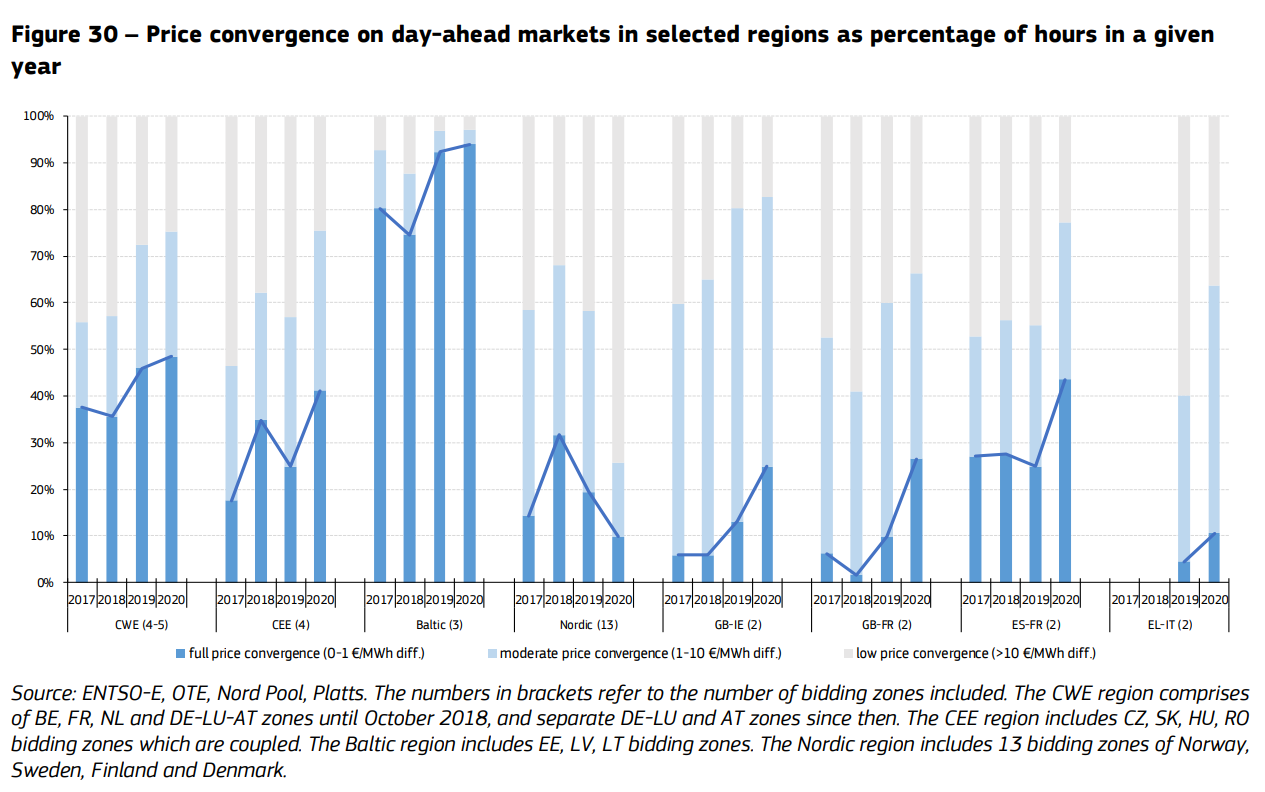
\includegraphics[height = 0.7\textheight]{figures/convergence.PNG}
        \\ Source: \cite{Report2019}
    \end{figure}
\end{frame}

\begin{frame}{Empirical: \citeauthor{Bockers2014} (\citeyear{Bockers2014})}
    \textbf{Empirical analysis of convergence between 2004 and 2011}

    \begin{itemize} \setlength\itemsep{1.5em}
              \pause \item Only partial convergence (mostly Germany-Austria)
              \pause \item Lack of convergence is not due to supply shocks
              \pause \item ``No theoretical model of effects of shocks in some countries on energy markets in neighboring countries''
    \end{itemize}

\end{frame}

\begin{frame}{Rational Expectations: \citeauthor{Gebhardt2013} (\citeyear{Gebhardt2013})}
    \textbf{Why is there no convergence in EU local electricity prices?}

    \begin{itemize} \setlength\itemsep{1.5em}
              \pause \item Rational producers and traders
              \pause \item Information asymmetries between local markets \pause
    \end{itemize}

    $\implies$ traders fail to engage and equalize prices

    Issues with the model...

    \begin{itemize} \setlength\itemsep{1.5em}
        \item ``our results highlight an additional advantage of \textit{market coupling}, i.e., integrating the national wholesale markets''
        \item ``we assumed that (...) cross-border trades do not influence the spot prices''
    \end{itemize}

\end{frame}

\begin{frame}{ABM: \citeauthor{Weidlich2008} (\citeyear{Weidlich2008})}

    \begin{columns}[T,onlytextwidth]

        \begin{column}{.4\textwidth}
            \begin{itemize} \setlength\itemsep{1.5em}
                \item Fixed demand side \pause
                \item Focus on market power \pause
                \item Agents ``learn'' the price mechanism \pause
                \item Neglected cross-border markets
            \end{itemize}
        \end{column}

        \hfill

        \begin{column}{.6\textwidth}
            \centering
            \resizebox{0.7\textwidth}{!}{\tikzstyle{basic} = [
draw,circle,
minimum size=10pt,
]

\tikzstyle{core} = [
draw,circle,
minimum size=10pt,
prosumer,
fill=prosumer,
text=black
]

\begin{tikzpicture}[-{Latex[scale=1]}, thick]

    \node [core] (1) {Consumers};
    \node [core, below = 4cm of 1] (3) {Producers};
    \node [basic, right = 1cm of 1] (2-1) {\makecell[c]{Constant \\ demand}};
    \node [basic, right = 1cm of 3] (4) {\makecell[c]{Market \\ power}};
    \node [basic, above = 1cm of 4] (2-2) {Supply};
    \node [basic, below right = 1cm and 2cm of 2-1] (5) {Prices};


    \path
    (1) edge (2-1)
    (4) edge (2-2)
    (3) edge (4)
    (2-2) edge (5)
    (2-1) edge [dashed, -] (5)
    ;

\end{tikzpicture}}
        \end{column}
    \end{columns}

\end{frame}

\begin{frame}{This paper}
    \begin{itemize} \setlength\itemsep{1.5em}
        \item Link between cross-border and local prices (network structure)
        \item Agent based model (bounded rationality)
        \item Role of demand shocks (prosumers)
    \end{itemize}
\end{frame}

\begin{frame}{What is new?}

    Comparison with previous ABM (\cite{Weidlich2008})
    \vfill

    \begin{columns}[T,onlytextwidth]

        \begin{column}{.4\textwidth}
            \centering
            \resizebox{\textwidth}{!}{\tikzstyle{basic} = [
draw,circle,
minimum size=10pt,
]

\tikzstyle{core} = [
draw,circle,
minimum size=10pt,
prosumer,
fill=prosumer,
text=black
]

\begin{tikzpicture}[-{Latex[scale=1]}, thick]

    \node [core] (1) {Consumers};
    \node [core, below = 4cm of 1] (3) {Producers};
    \node [basic, right = 1cm of 1] (2-1) {\makecell[c]{Constant \\ demand}};
    \node [basic, right = 1cm of 3] (4) {\makecell[c]{Market \\ power}};
    \node [basic, above = 1cm of 4] (2-2) {Supply};
    \node [basic, below right = 1cm and 2cm of 2-1] (5) {Prices};


    \path
    (1) edge (2-1)
    (4) edge (2-2)
    (3) edge (4)
    (2-2) edge (5)
    (2-1) edge [dashed, -] (5)
    ;

\end{tikzpicture}}
        \end{column}

        \hfill

        \begin{column}{.57\textwidth}
            \centering
            \resizebox{\textwidth}{!}{\tikzstyle{basic} = [
draw,circle,
minimum size=10pt
]

\tikzstyle{core} = [
draw,circle,
minimum size=10pt,
prosumer,
fill=prosumer,
text=black
]


\begin{tikzpicture}[-{Latex[scale=1]}, thick]

    \node [core] (1) {Prosumers};
    \node [core, below = 4cm of 1] (3) {Producers};
    \node [basic, right = 1cm of 1] (2-1) {\makecell[c]{Demand \\ shocks}};
    \node [basic, right = 1cm of 3] (4) {\makecell[c]{Market \\ power}};
    \node [basic, above = 1cm of 4] (2-2) {\makecell[c]{Supply \\ shocks}};
    \node [basic, below right = 1cm and 2cm of 2-1] (5) {Prices};
    \node [basic, right = 1cm of 4] (7) {\makecell[c]{Bargaining \\ power}};
    \node [core, right = 1cm of 7] (6) {Providers};


    \path
    (1) edge (2-1)
    (4) edge (2-2)
    (3) edge (4)
    (2-2) edge (5)
    (2-1) edge (5)
    (6) edge (7)
    (7) edge (4) 
    ;

\end{tikzpicture}}
        \end{column}
    \end{columns}

\end{frame}

\section{Overview}

\begin{frame}{Research question}

    \begin{itemize} \setlength{\itemsep}{1em}
        \item How do exogenous and unexpected demand shocks affect the price formation mechanism? \pause
        \item How do shock in prices transmit to the cross-border market? \pause
        \item Can this shock produce sustained price imbalances? \pause
        \item Are current policies effective in this framework?
    \end{itemize}

\end{frame}


\begin{frame}{Results}
    \begin{itemize} \setlength\itemsep{1.5em}
              \pause \item Bargaining power determines price contagion (bigger and more ``central'' markets)
              \pause \item Demand shocks cause \textbf{hysteresis}: sustained price imbalances - implications for prosumers
              \pause \item This implies: markets integration is not sufficient
    \end{itemize}
\end{frame}

\section{Model}

\begin{frame}{Model outline}
    \centering
    \resizebox{\textwidth}{!}{\tikzstyle{var} = [
draw,circle,
prosumer,
fill=prosumer,
text=black,
minimum size=10pt]

\tikzstyle{agent} = [
draw, circle,
fill=blue!30,
minimum size=10pt]

\tikzstyle{derived} = [
draw, circle, dashed,
minimum size=10pt]

\tikzstyle{time} = [
draw=gray, rectangle,
dashed,
thick,
inner sep=5pt]

\tikzstyle{market} = [
draw=gray, circle,
dashed,
thick,
inner sep=5pt]


\begin{tikzpicture}[-{Latex[scale=1]}, thick, every text node part/.style={align=center, fontscale=0.8}]

    \node [agent] (prov) {Provider};
    \node [market, left = 2cm of prov] (cb-market) {Cross-border \\ market};
    \node [agent, above right = 1cm and 5cm of prov] (prod) {Producers};
    \node [agent, below right = 1cm and 5cm of prov] (pros) {Prosumers};
    \node [market, right = 2cm of prov] (w-market) {Local \\ wholesale \\ market};

    \path
    (cb-market) edge [bend left] node [above] {$Y_t$} (prov)
    (prov) edge [dashed, bend left] node [below] {$P_t$} (cb-market)
    (prov) edge [ bend left] node [above] {$X_t$} (w-market)
    (w-market) edge [dashed, bend left] node [below] {$p_t$} (prov)
    (prod) edge [] node [above left] {$S_t$} (w-market)
    (w-market) edge [{Latex[scale=1]}-{Latex[scale=1]}] node [below left] {$e_t \  M$} (pros)
    ;

\end{tikzpicture}}
\end{frame}

\begin{frame}
    Prosumers...
    \begin{itemize} \setlength\itemsep{1.5em}
              \pause \item ...demand $e_t$ which can be either low ($\underline{e}$) or high ($\overline{e}$)
              \pause \item ...a ``demand shock'' is a period of $\overline{e}$
    \end{itemize}
\end{frame}


\begin{frame}

    Producers...
    \begin{itemize} \setlength\itemsep{1.5em}
              \pause \item ...make delayed production decision $s_{t+1} = s_t + \underbrace{r_t(s_t, p_t)}_{\text{policy}}$
              \pause \item ...believe price to be constant $\B_t[p_{t+1}] = p_t$
              \pause \item ...unit production cost $k$ and marginal cost of ramp-up $\max\{0, s_t r_t\}$
    \end{itemize}

\end{frame}

\begin{frame}
    If $mc = mb$, $\frac{\partial r}{\partial p_t} \propto \sqrt{p_t}$ and $\frac{\partial r}{\partial s_t} \propto - s_t$

    \begin{figure}
        \includegraphics[width=0.75\linewidth]{../../plots/rfunction.pdf}
    \end{figure}
\end{frame}

\begin{frame}
    \visible<1->{
        Local markets can have \textbf{excess demand} $X$ which evolves as,

        \begin{equation*}
            X_{t+1} - X_t = \overbrace{M (e_{t+1} - e_t)}^{\text{change in demand}} - \overbrace{R_t}^{\text{change in supply }\sum_{i, t} r_{i, t}}
        \end{equation*}
    }

    \visible<2->{
        Providers form believes over

        \begin{equation*}
            \B_t[e_{t+1}] = e_t
        \end{equation*} and

        \begin{equation*}
            \B_t \left[R_t(p_t, S_t) \right] = \alpha_t + \gamma_t \ \underbrace{p_t}_{\text{local price}} + \eta_t \ \underbrace{S_t}_{\text{local supply}}
        \end{equation*} updated via WLS.
    }
\end{frame}

% CB market
\begin{frame}{Providers: link between local and cross-border markets}
    \begin{columns}[T,onlytextwidth]

        \begin{column}{.4\textwidth}
            \begin{equation*}
                \begin{split}
                    &V(X_t, S_t) = \max_{p_t, \Y_t} \\
                    & \overbrace{p_t X_t}^{\text{local revenue}} -  \overbrace{\sum_{j \in N_{\mathcal{A}}(i)} Y^j_t P^j(\Y_t)}^{\text{cost of buying abroad}} + \\
                    &\lambda_t \underbrace{\left( X_t - \sum_{j \in N_{\mathcal{A}}(i)} Y^j_t\right)}_{\text{matching constraint}}  + \beta  V(X_{t+1}, S_{t+1})
                \end{split}
            \end{equation*}
        \end{column}

        \hfill

        \begin{column}{.5\textwidth}
            \centering
            \resizebox{\textwidth}{!}{\tikzstyle{prosumers} = [
draw,circle,
prosumer,
fill=prosumer,
text=black,
minimum size=5pt]

\tikzstyle{provider} = [
draw,circle,
minimum size=10pt]

\tikzstyle{market} = [
draw=gray, dashed, thick,
inner sep=8pt]


\begin{tikzpicture}[{Latex[scale=0.5]}-{Latex[scale=0.5]}, thick]

    % Placing providers
    \foreach \x/\y [count=\j] in {1/1, -1/1, 1/-1, -1/-1}
        % Draw provider
        {\node [provider]  (\j) at (2*\x, 2*\y) [fontscale=0.8] {\makecell[l]{Prov. \j \\ $X(p_{\j})$}};

            % Draw prosumers
            \edef\points{}
            \foreach \z/\w [count=\i] in {0/2, 1/2.1, 1.75/1.75, 2.1/1, 2/0}
                {\node [prosumers] (\x\y\i) at (\x + 1.3*\x*\z, \y + 1.5*\y*\w) [fontscale=0.6] {$x_{\i}$};
                    \path (\j) edge [] node [fontscale = 0.6] {} (\x\y\i);
                    \xdef\points{(\x\y\i) \points}
                };}

    \path
    (1) edge [-{Latex}] node [above, fontscale=0.8] {$Y^{(1, 2)}$} (2)
    (1) edge [-{Latex}] node [right, fontscale = 0.8] {$Y^{(1, 3)}$} (3)
    (1) edge [-{Latex}] node [above left, fontscale = 0.8] {$Y^{(1, 4)}$} (4)
    (3) edge [-{Latex}] node [above, fontscale = 0.8] {$Y^{(3, 4)}$} (4);

\end{tikzpicture}}
        \end{column}

    \end{columns}
\end{frame}


\begin{frame}

    The optimization problem determines the \textbf{local price evolution}
    \begin{equation*}
        p_{i, t+1} - p_{i, t} = \underbrace{L_{i, t}(X_{i, t}, S_{i, t})}_{\text{optimization in local market}} + \overbrace{2 P(\Y_t)}^{\text{influence of cross-border market}}
    \end{equation*}

    \begin{itemize} \setlength\itemsep{1.5em}
        \item Cross-border and local markets link (addressing \citeauthor{Gebhardt2013})
        \item Determines: shock of neighbor $\xrightarrow{}$ local prices (addressing \citeauthor{Bockers2014})
        \item Note that if $L_{i, t} = 0$ and $P = 0$, then $\B_t[p_{t+1}] = p_t = p_{t+1}$
    \end{itemize}

\end{frame}

\begin{frame}{Local policy: $L_{i, t}(X_{i, t}, S_{i, t})$}
    $L_{i, t}$ for ``true'' beliefs $(\alpha_t, \gamma_t, \eta_t)$
    \begin{figure}
        \includegraphics[width=0.7\linewidth]{../../plots/pricingnonbinding.pdf}
    \end{figure}
\end{frame}

\begin{frame}{Nash-bargaining in the cross-border market: $P(\Y_t)$}
    Given $X_{i, t}$ and $p_{i, t}$, Nash-bargaining solution of trading price

    \begin{equation*}
        P_t^{(i, j)} = \arg \max \{  \text{joint profits of $i$ and $j$} \}
    \end{equation*}

    Depends on

    \begin{itemize} \setlength\itemsep{1.5em}
        \item Local revenue difference $\Delta^{(i, j)}_t = X_{i, t} p_{i, t} - X_{j, t} p_{j, t} $
        \item Outside options of $i$ and $j$, respectively $\sum_m Y_t^{(i, m)} P_t^{(i, m)}$ and $j$ $\sum_l Y_t^{(j, l)} P_t^{(j, l)}$
    \end{itemize}

\end{frame}

\begin{frame}

    \begin{equation*}
        P_t^{(i, j)} = \frac{1}{2 \ Y_t^{(i, j)}}  \left(\Delta^{(i, j)}_t + \underbrace{\sum_{m} Y_t^{(j, m)} \  P_t^{(j, m)}}_{\text{outside option of } j} - \underbrace{\sum_{l} Y_t^{(i, l)} \  P_t^{(i, l)}}_{\text{outside option of } i} \right)
    \end{equation*}


    Takeaways for demand shocks...

    \begin{itemize} \setlength\itemsep{1.5em}
              \pause \item Contemporaneous effect analytically: $X_{j, t} \xrightarrow{} \Delta^{(i, j)}_t \xrightarrow{} P_t^{(i, j)} \xrightarrow{} p_{i, t}$
              \pause \item Delayed effect via simulation: $p_{i, t}  \xrightarrow{} X_{i, t+1} \xrightarrow{} \Y_t$
              \pause \item \textbf{Network structure}, via the outside options, crucial for \textbf{contagion}
    \end{itemize}

\end{frame}

\section{Contagion}

\begin{frame}{Looking at $P$ as a whole}
    Stack all variables in vectors of size $\lvert edges \rvert$. Use the line-graph operator of the original network $L(network)$ with adjacency matrix $\matr{G}$.

    \begin{equation*}
        \begin{split}
            network &= (nodes, edges) \\
            L(network) &= (edges, \subseteq nodes)
        \end{split}
    \end{equation*}

    \begin{equation*}
        L\Big(  \resizebox{0.3\linewidth}{!}{\tikzstyle{node} = [
draw,circle,
minimum size=40pt]

\begin{tikzpicture}[-{Latex[scale=1]}, thick, baseline={([yshift=-.5ex]current bounding box.center)}]

    \node [node] (one) {$1$};
    \node [node, right = 2cm of one] (two) {$2$};
    \node [node, right = 2cm of two] (three) {$3$};


    \path
    (one) edge [] node [above] (onetwo) {$(1, 2)$} (two)
    (two) edge [] node [above] (twothree) {$(2, 3)$} (three)
    ;
    

\end{tikzpicture}} \Big) = \resizebox{0.3\linewidth}{!}{\tikzstyle{node} = [
draw,circle,
minimum size=40pt]

\begin{tikzpicture}[-{Latex[scale=1]}, thick, baseline={([yshift=-.5ex]current bounding box.center)}]

    \node [node, below = 1cm of onetwo] (one-two) {$(1, 2)$};
    \node [node, below = 1cm of twothree] (two-three) {$(2, 3)$};

    \path (one-two) edge [] node [above] {$2$} (two-three);
    

\end{tikzpicture}}
    \end{equation*}
\end{frame}

\begin{frame}{Bargaining influence matrix}

    Stacking in vectors,

    \begin{equation*}
        \begin{split}
            2(P_t \circ \Y_t) &= \Delta_t  - \G \left( P_t \circ \Y_t \right) \\
            (2\I + \G) (P_t \circ \Y_t) &= \Delta_t  \\
            (P_t \circ \Y_t) &= (2\I + \G)^{-1} \Delta_t
        \end{split}
    \end{equation*}

    Contagion is determined, via $P(\Y_t)$, by

    \begin{equation*}
        (2\I + \G)^{-1}
    \end{equation*}

    called here \textit{bargaining influence matrix}

\end{frame}

\begin{frame}{Star}

    If $\mathcal{A}$ (\textit{left}) is a star graph then $L(\mathcal{A})$ (\textit{right}) is a complete graph. \vspace{5mm}

    \begin{columns}[T,onlytextwidth]

        \begin{column}{.46\textwidth}
            \resizebox{\linewidth}{!}{\tikzstyle{var} = [
draw,circle,
minimum size=10pt]

\tikzstyle{agent} = [
draw, circle,
minimum size=10pt]

\begin{tikzpicture}[-{Latex[scale=1]}, thick]

    \node [agent] (one) {Prov. $1$};
    \node [agent, left = 3cm of one] (two) {Prov. $2$};
    \node [agent, above = 3cm of one] (three) {Prov. $3$};
    \node [agent, right = 3cm of one] (four) {Prov. $4$};


    \path
    (one) edge [] node [above] {$Y^{(1, 2)}$} (two)
    (one) edge [] node [left] {$Y^{(1, 3)}$} (three)
    (one) edge [] node [above] {$Y^{(1, 4)}$} (four);

\end{tikzpicture}}
        \end{column}

        \hfill

        \begin{column}{.46\textwidth}
            \resizebox{\linewidth}{!}{\tikzstyle{var} = [
draw,circle,
minimum size=10pt]

\tikzstyle{agent} = [
draw, circle,
minimum size=10pt]

\begin{tikzpicture}[-, thick]

    \node [agent] (one-two) {$(1, 2)$};
    \node [agent, above right = 1cm and 1cm of one-two] (one-three) {$(1, 3)$};
    \node [agent, below right = 1cm and 1cm of one-three] (one-four) {$(1, 4)$};
    \node [agent, below right = 1cm and 1cm of one-two] (one-n) {$(1, n)$};


    \path
    (one-two) edge [] node {} (one-three)
    (one-two) edge [] node {} (one-four)
    (one-three) edge [] node {} (one-four)
    (one-two) edge [] node {} (one-n)
    (one-three) edge [] node {} (one-n)
    (one-four) edge [] node {} (one-n);

\end{tikzpicture}}
        \end{column}
    \end{columns}
\end{frame}

\begin{frame}{Path}
    If $\mathcal{A}$ (\textit{left}) is a path graph then $L(\mathcal{A})$ (\textit{right}) is a path graph. \vspace{5mm}

    \begin{columns}[T,onlytextwidth]

        \begin{column}{.46\textwidth}
            \resizebox{\linewidth}{!}{\tikzstyle{var} = [
draw,circle,
minimum size=10pt]

\tikzstyle{agent} = [
draw, circle,
minimum size=10pt]

\begin{tikzpicture}[-, thick]

    \node [agent] (one) {Prov. $1$};
    \node [agent, below right = 2cm and 2cm of one] (two) {Prov. $2$};
    \node [agent, below right = 2cm and 2cm of two] (three) {Prov. $3$};
    \node [agent, below right = 2cm and 2cm of three] (four) {Prov. $n$};


    \path
    (one) edge [] node [below left] {$Y^{(1, 2)}$} (two)
    (two) edge [] node [below left] {$Y^{(2, 3)}$} (three)
    (three) edge [dashed] node [below left] {} (four);

\end{tikzpicture}}
        \end{column}

        \hfill

        \begin{column}{.46\textwidth}
            \resizebox{\linewidth}{!}{\tikzstyle{var} = [
draw,circle,
minimum size=10pt]

\tikzstyle{agent} = [
draw, circle,
minimum size=10pt]

\begin{tikzpicture}[-{Latex[scale=1]}, thick]

    \node [agent] (one-two) {$(1, 2)$};
    \node [agent, below right = 2cm and 2cm of one-two] (two-three) {$(2, 3)$};
    \node [agent, below right = 2cm and 2cm of two-three] (three-four) {$(3, 4)$};
    \node [agent, below right = 2cm and 2cm of three-four] (last) {$(n, n-1)$};


    \path
    (one-two) edge [] node [below left] {Prov. $2$} (two-three)
    (two-three) edge [] node [below left] {Prov. $3$} (three-four)
    (three-four) edge [dashed] (last);

\end{tikzpicture}}
        \end{column}
    \end{columns}
\end{frame}


\begin{frame} {Bargaining influence matrix: $(2\I + \G)^{-1}$ }

    \begin{columns}
        \begin{column}{.47\textwidth}
            \begin{figure}
                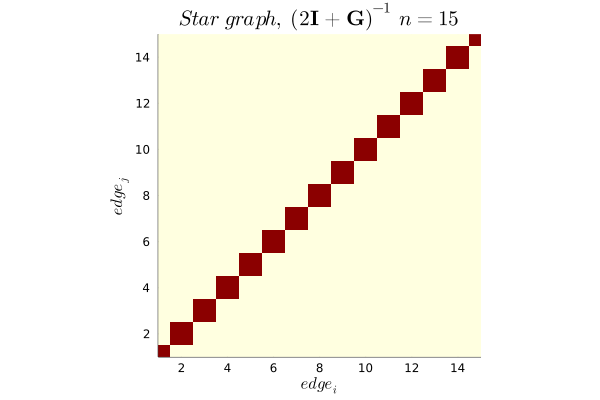
\includegraphics[width = \linewidth]{../../plots/bargmatrices/star.pdf}
                \\ ...in the star graph
            \end{figure}
        \end{column}
        \begin{column}{.47\textwidth}
            \begin{figure}
                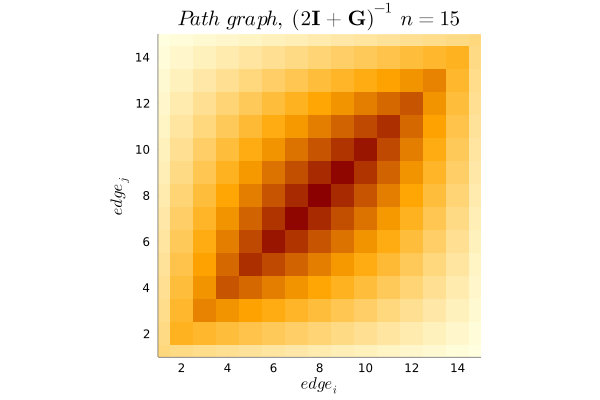
\includegraphics[width = \linewidth]{../../plots/bargmatrices/path.pdf}
                \\ ...in the path graph
            \end{figure}
        \end{column}
    \end{columns}

\end{frame}

\begin{frame} {Policy function $p_{t+1}$ of the central node}
    \begin{columns}
        \begin{column}{.47\textwidth}
            \begin{figure}
                \includegraphics[width = \linewidth]{../../plots/pricing.pdf}
                \\ ...in the star graph
            \end{figure}
        \end{column}
        \begin{column}{.47\textwidth}
            \begin{figure}
                \includegraphics[width = \linewidth]{../../plots/pricingpath.pdf}
                \\ ...in the path graph
            \end{figure}
        \end{column}
    \end{columns}
\end{frame}

\begin{frame}{Star: central demand shock simulation}
    \begin{figure}[H]
        \centering
        \includegraphics[height = 0.8\textheight]{\plotpath/central/star/pricesupply.pdf}
    \end{figure}

\end{frame}

\begin{frame} {Path: central demand shock simulation}
    \begin{figure}[H]
        \centering
        \includegraphics[height = 0.8\textheight]{\plotpath/central/path/pricesupply.pdf}
    \end{figure}
\end{frame}

\begin{frame}{Policy evaluation: ``market coupling''}
    \begin{itemize}
        \item Market coupling works only if it reduces bargaining power concentration \pause
        \item ``Flatten the policy function'' \pause
    \end{itemize}

    Let the spread of bargaining power be defined as

    \begin{equation*}
        \rho = \left(\frac{\sigma}{\mu}\right)_{(2\I + \G)^{-1}}
    \end{equation*}

    A low $\rho$ implies diffuse bargaining power and ``flat'' policy function
\end{frame}

\begin{frame}[allowframebreaks]{More path, less star}

    \centering
    \resizebox{0.7\textwidth}{!}{\tikzstyle{var} = [
draw,circle,
minimum size=10pt]

\tikzstyle{agent} = [
draw, circle,
minimum size=10pt]

\begin{tikzpicture}[-{Latex[scale=1]}, thick]

    \node [agent] (one) {Prov. $1$};
    \node [agent, right = 2cm of one] (two) {Prov. $2$};
    \node [agent, left = 2cm of one] (three) {Prov. $3$};
    \node [agent, below = 2cm of one] (four) {Prov. $4$};

    \node [agent, left = 2cm of four] (five) {Prov. $5$};


    \path
    (one) edge (two)
    (one) edge (three)
    (one) edge (four);

    \path
    (four) edge [dashed] node [below] {$\rho$ decreases} (five)
    (one) edge [dashed] node [above left] {$\rho$ increases} (five);

\end{tikzpicture}}



    \begin{figure}
        \includegraphics[width = 0.8\linewidth]{\plotpath/blackouts/rhos.pdf}
        \\ $\rho$ for different graphs and sizes
    \end{figure}

\end{frame}

\section{Conclusion}

\begin{frame}{Takeaways}
    \begin{itemize} \setlength\itemsep{1.5em}
        \item Market power and rational expectations are not adequate frameworks \pause
        \item Demand shocks can create sustained imbalances (prosumers) \pause
        \item Further market integration needs to address ``bargaining power''
    \end{itemize}
\end{frame}

\begin{frame}{What's next}
    \begin{itemize} \setlength\itemsep{1.5em}
        \item Further questions: \pause
              \begin{itemize} \setlength\itemsep{1em}
                  \item What if prosumers sell electricity ($e_t < 0$)? \pause
                  \item What if markets have different sizes ($M$ and $N$)? \pause
              \end{itemize}
        \item Model improvements: \pause
              \begin{itemize} \setlength\itemsep{1em}
                  \item Bipartite graphs of buyers and seller \pause
                  \item Simplify producers further and focus on providers bargaining procedure \pause
              \end{itemize}
        \item Model calibration
    \end{itemize}
\end{frame}


\begin{frame}[allowframebreaks]{Bibliography}
    \printbibliography
\end{frame}

\end{document}